\documentclass[a4paper]{article}
\usepackage[paperwidth=17cm, paperheight=22.5cm, bottom=2.5cm, right=2.5cm]{geometry}
\usepackage[spanish]{babel}
\usepackage[utf8]{inputenc} %Paquete para escribir acentos y otros símbolos directamente
%\usepackage{enumerate}
\usepackage{graphicx}
%\usepackage{subfig} %para poner subfiguras
\graphicspath{{Img/}} %En qué carpeta están las imágenes


\begin{document}

%----------------------------------------------------------------------------------------
%	COMANDOS PERSONALIZADOS
%----------------------------------------------------------------------------------------
%	PORTADA
%----------------------------------------------------------------------------------------

\title{TÍTULO DE LA TESIS} %Con este nombre se guardará el proyecto en writeLaTex

\begin{titlepage}
\begin{center}

\textsc{\huge \textbf{MEMORIA DE PRÁCTICAS}}\\[1em]

%Figura
\begin{figure}[h]
\begin{center}

\includegraphics[width=0.5\textwidth]{facu.jpg}
\end{center}
\end{figure}

\vspace{1em}

\textsc{\huge \textbf{PROYECTO DE SERVICIOS TELEMÁTICOS AVANZADOS}}\\[1em] 



\textsc{\Large MARÍA TERESA MORENO BOLUDA}\\[1em]

\textsc{\Large JUAN ÁNGEL SÁNCHEZ LÓPEZ}\\[1em]

\vspace{3em}

\begin{large}
Supervisado por: \\
Gabriel López Millán \\ Alejandro Molina Zarca
\end{large}

\end{center}



\vspace*{\fill}
\textsc{Murcia. \hspace*{\fill} Convocatoria Enero.}

\end{titlepage}





%--------------------------
%	TABLA DE CONTENIDOS
%--------------------------

\thispagestyle{empty}
\tableofcontents
\newpage
%---------------------
 %empieza la numeración de las páginas


\section{Definición de la Topología Real}

Para llevar a cabo el desarrollo de esta práctica el primer paso a seguir es el establecimiento de los servicios, relaciones y funcionalidades que debe de tener cada una de las tres topologías presentes en el escenario realizado. 

\noindent Nuestro escenario está ligado a las administraciones de las conserjerías de cada gobierno autonómico

\medskip
\noindent La topología ideal se muestra en la Figura 1:0, como podemos observar se consta de tres organizaciones distintas conectadas entre sí a través de internet. Dos de estas organizaciones presentan la misma estructura de despliegue. La organización 110, en nuestro caso, se corresponderá con la sede principal del escenario dado que es la que consta de una
mayor cantidad de servicios desplegados y las organizaciones 111 y 112 representan el despliegue de dos organizaciones gestionadas por la primera.

   
// figura de la topología ideal 

\medskip 
\noindent Una vez presentada la topología ideal, nos centraremos en explicar 

.........

\noindent En la topología se debe desplegar una serie de servicios telemáticos, así como se deberá proteger el acceso a éstos y la transmisión de los paquetes de forma posterior al despliegue.  Concretamente la topología debe incluir los servicios de monitorización de los dispositivos de la red a través del protocolo SNMP, un servicio de almacenamiento de información en la nube mediante el despliegue de onwcloud, llamadas sobre voIP para
lo que se llevará a cabo el despliegue del servicio asterisk y un directorio activo para la autenticación en los servicios de owncloud y asterisk mediante LDAP.

\medskip
\noindent Dados los servicios que se deben desplegar supondremos que serán implementados en las conserjerías de cada gobierno autonómico, en concreto, en la Región de Murcia y la Comunidad Valenciana. Dichas conserjerías estarán gestionadas por un departamento central que se encargará de la administración de red y de solucionar cualquier avería que pueda ocurrir en ambas conserjerías. Se ha elegido este escenario real por la necesidad de almanamiento en la nube para la disponibilidad de compartición de documentos en la nube o la necesidad de repositorio de almacenamiento para los usuarios de estas organizaciones así como la implementación de una comunicación vía voIP entre las conserjerías y el departamento central para el abaratamiento de coste de las llamadas entre ellos, ya que no se necesita
incurrir en un gasto adicional de líneas telefónicas.

\medskip
\noindent La organización 110, llamada departamento central, constará de la implementación y despliegue funcional de los servicios de monitorización de red, cloud, voIP y del directorio activo que será utilizado por las dos conserjerías para el acceso al servicio cloud.

\medskip
\noindent En el caso de las organizaciones 111 y 112, conserjería de Murcia y Valencia respectivamente, se consta del despliegue del servicio de monitorización y de voIP. Para que ambas tengan acceso a los datos de forma conjunta se va a permitir el acceso al servicio cloud desplegado en la organización principal. La centralización de la información supone un riesgo de cara a recibir ataques que comprometan la información que los usuarios transmitirán o solicitarán al cloud con lo que la idea principal será establecer un tunelado IPSec para que dicha información no
se transmita a través de la red en claro. En el caso de asterisk suponemos que la red interna de ambas organizaciones es segura y no requerirá incluir un cifrado de la información transmitida desde el cliente a la centralita y viceversa.


\newpage

\section{Protocolo SNMP}
El protocolo SNMP (Simple Network Management Protocol) consiste en la monitorización de los distintos componentes de una red. Dentro de este protocolo encontramos dos roles posibles, el rol de agente que será el que asume el dispositivo manejado y el de manejador que se encargará de solicitar la información de monitorización al agente.

\medskip
\noindent En nuestro escenario ideal se ha aplicado la versión 2 de éste protocolo. Hemos decidido esto porque las organizaciones están conectadas entre sí mediante un túnel VPN, por lo que entre ellas solo se generará tráfico interno y no será necesario la securización de SNMP versión 3. 

\medskip
\noindent La versión 2 del protocolo SNMP se caracteriza por la inclusión de nuevos comandos de interés como getbulk para recuperar información en grandes cantidades y mejora de funcionalidad de la primera versión como en el caso de los trap.

\medskip
\noindent Los trap son mensajes lanzados por el agente para notificar de situaciones de error o excepcionales, en el caso de la versión 2 lo que se ha hecho ha sido mejorar su función
ya que estaban disponibles en la primera.

\medskip
\noindent En el caso de la operación getbulk se incluye con el fin de mejorar la obtención de información por parte del manejador ya que, de este modo, puede obtener grandes cantidades de información con una única solicitud, a diferencia de la primera versión.

\medskip
\noindent Los MIB o Management Information Base, son estructuras jerárquicas que contienen la información de todos los dispositivos gestionados a través de este protocolo. Los arboles de información SNMP constan de dos tipos distintos de nodos: estructurales o de información. Los nodos estructurales no contienen información útil del sistema sino que almacenan su posición en el árbol, son ramas del árbol. En cambio los nodos de información son nodos hoja, estos nodos se basan en la macro object-type que contiene cláusulas para la definición de características de un MIB, es decir, se encargan de definir los tipos de datos de los MIB.

\medskip
\noindent SNMPv2 se compone de los siguientes nodos estructurales: system, interfaces, at, ip, icmp, tcp, udp, egp y translation.
Del nodo System cuelga información genérica del sistema gestionado como la información de localización o el nombre. 

\subsection{Definición de usuarios}
\subsection{Fichero de configuración}
\subsection{Análisis de trazas}

\newpage
\section{Protocolo de voz sobre IP}

A continuación, vamos a desplegar un servicio de VoIP basado en el uso de Asterisk y SIP en todas las organizaciones.
La VoIP intenta emular a la telefonía tradicional. Mientras que en ésta el envío del audio se realiza de forma analógica a través de unos circuitos virtuales, en la VoIP el audio es enviado digitalmente como paquetes de datos sobre el protocolo IP.

\medskip
\noindent En una llamada de VoIP diferenciamos las siguientes etapas:
\begin{itemize}
    \item El establecimiento de la llamada que enviará ese audio (SIP).
    \item La conversión del audio analógico en digital (códecs).
    \item El envío de ese audio por la red desde un origen hasta un destino (RTP).

\end{itemize}

\subsection{Protocolo SIP}
El protocolo SIP, Session Iniciation Protocol, es un protocolo de señalización end-to-end. Permite establecer una llamada entre dos usuarios sobre una red IP, negociando las características de la misma. Sin embargo, la función de SIP es únicamente de sincronización, puesto que no transporta audio ni garantiza la calidad del uso de este protocolo de transporte. 

\medskip
\noindent SIP se encarga de establecer la conexión entre los equipos y de establecer las características que tendrá la llamada, pero no garantiza que la red pueda soportar las características establecidas.
Para implementarlo, los equipos finales implementan dos Agentes SIP diferentes: User Agent Client (UAC), y User Agent Server (UAS). El primero se utiliza para realizar solicitudes de llamadas, es decir, para realizar una llamada. Y el segundo para recibirlas.

\medskip
\noindent
Además, se diferencian tres tipos de Servidores:

\begin{itemize}
    \item Por un lado, el Proxy Server y el Redirect Server que se encargan de proporcionar la información necesaria para que la llamada llegue hasta el destinatario (el proxy server redirige la llamada directamente, mientras que el Redirect Proxy indica la IP en la que se encuentra el destinatario).
    
    \item Por otro lado, el Registrer Server acepta solicitudes de registro de usuarios, y mantiene la localización de los mismos en un Servidor de Localización (Location Server). El Registrer Server se puede localizar en la misma máquina que el Proxy/Redirect o en otra distinta. 
    
\end{itemize}  

\noindent
Todos los terminales se registran, nada más iniciarse, en el Register Server, donde se asocia su ID de usuario con su IP. De esta forma, al realizar una llamada, los proxys buscan la IP del equipo al que queremos llamar, o nos redirigen directamente hacia él (Proxy Server), o nos indica la IP (Redirect Server).
Una vez que ya conocemos la IP del equipo al que queremos llamar, entra en juego el protocolo SIP propiamente dicho. 

\begin{figure}[h]
    \begin{center}
        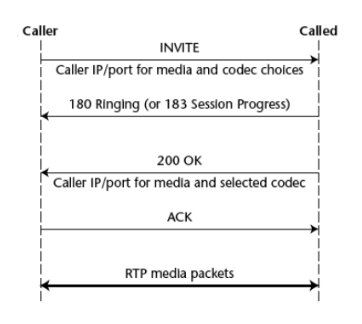
\includegraphics[width=0.7\textwidth]{sip-register.jpg}
         \caption{Negociación básica SIP.}
        
    \end{center}
    \label{fig:1}
\end{figure}

En la figura \ref{fig:1} podemos ver un ejemplo de una negociación básica SIP.

\subsection{Protocolo RTP}

\subsection{Diseño ideal}
\subsection{Diseño implementado}
\subsection{Análisis de trazas}

\section{Servicio de directorio activo, LDAP}
\subsection{Integración LDAP con Asterisk}
\subsection{Análisis de trazas}

\section{Servicio de almacenamiento, Owncloud}
\subsection{Establecimiento de conexión segura}
\subsection{Cuotas de disco de usuarios}
\subsection{Revocación de certificados}
\subsection{Cifrado}
\subsection{Autenticación de owncloud con LDAP}

\section{Seguridad adicional}
\subsection{Seguridad en Owncloud}

\section{Bibliografía}
%----------------------------------------------------------------------------------------
%	BIBLIOGRAFÍA
%----------------------------------------------------------------------------------------
\backmatter
\nocite{*}
\bibliographystyle{plain}
\bibliography{bibliografía.bib} %Aquí ponen el nombre del archivo .bib






\end{document}